\documentclass[11pt]{report}
\usepackage[utf8]{inputenc}
\usepackage{graphicx}
\usepackage{amsmath}
\usepackage{booktabs}
\usepackage{longtable}
\usepackage{float}
\usepackage[a4paper, top=2.5cm, bottom=2.5cm, left=2.5cm, right=2.5cm]{geometry}

\title{
    \vspace{2cm}
    \textbf{Machine Learning 441: Assignment 1} \\
    \large Data Exploration
}
\author{
    Ruan Buhr \\ 
    \small 26440873
}
\date{\today}

\begin{document}

\maketitle

\section*{Task 1: Data Quality Reports}

The \texttt{badDataSet.csv} data set contains 581012 instances, with 62 descriptive features and a single response.

\begin{table}[H]
\centering
\caption{Data Quality Report for the Descriptive Features.}
\label{tab:data_quality_report_des_feat}
\resizebox{\textwidth}{!}{
    \begin{tabular}{lrrrrrrrrrr}
\toprule
Feature & Count & \% Miss. & Card. & Min. & 1st Qrt. & Mean & Median & 3rd Qrt. & Max. & Std. Dev. \\
\midrule
A1 & 581012 & 0.00 & 1978 & 2054845.65 & 3104928.15 & 3271134.43 & 3311628.60 & 3496222.05 & 4264440.30 & 309481.13 \\
A2 & 578069 & 0.51 & 361 & 0.00 & 58.00 & 155.66 & 127.00 & 260.00 & 360.00 & 111.91 \\
A3 & 581012 & 0.00 & 576099 & 0.00 & 145.49 & 389.92 & 318.12 & 652.53 & 903.48 & 280.34 \\
A4 & 580708 & 0.05 & 67 & 0.00 & 9.00 & 14.10 & 13.00 & 18.00 & 66.00 & 7.49 \\
A5 & 578069 & 0.51 & 569 & -691.00 & 108.00 & 269.42 & 218.00 & 384.00 & 1397.00 & 212.56 \\
A6 & 581012 & 0.00 & 581012 & -173.07 & 6.99 & 46.42 & 29.91 & 68.97 & 600.95 & 58.30 \\
A7 & 578069 & 0.51 & 577988 & -1.00 & -0.50 & -0.00 & -0.00 & 0.50 & 1.00 & 0.58 \\
A8 & 581012 & 0.00 & 5811 & 0.00 & 1106.00 & 8158.11 & 1997.00 & 3328.00 & 510165098.00 & 1185156.02 \\
A9 & 578069 & 0.51 & 207 & 0.00 & 198.00 & 212.14 & 218.00 & 231.00 & 254.00 & 26.77 \\
A10 & 578069 & 0.51 & 186 & 0.00 & 213.00 & 223.32 & 226.00 & 237.00 & 254.00 & 19.77 \\
A11 & 581012 & 0.00 & 255 & 0.00 & 119.00 & 142.53 & 143.00 & 168.00 & 254.00 & 38.27 \\
A12 & 578069 & 0.51 & 5826 & 0.00 & 1024.00 & 1980.43 & 1710.00 & 2550.00 & 7173.00 & 1324.25 \\
A13 & 578069 & 0.51 & 2 & 0.00 & 0.00 & 0.45 & 0.00 & 1.00 & 1.00 & 0.50 \\
A14 & 581012 & 0.00 & 2 & 0.00 & 0.00 & 0.05 & 0.00 & 0.00 & 1.00 & 0.22 \\
A15 & 581012 & 0.00 & 2 & 0.00 & 0.00 & 0.44 & 0.00 & 1.00 & 1.00 & 0.50 \\
A16 & 578069 & 0.51 & 1 & 0.00 & 0.00 & 0.00 & 0.00 & 0.00 & 0.00 & 0.00 \\
A17 & 581012 & 0.00 & 1 & 0.00 & 0.00 & 0.00 & 0.00 & 0.00 & 0.00 & 0.00 \\
A18 & 578069 & 0.51 & 3 & 0.00 & 0.00 & 0.07 & 0.00 & 0.00 & 2.00 & 0.28 \\
A19 & 581012 & 0.00 & 2 & 0.00 & 0.00 & 0.50 & 0.00 & 1.00 & 1.00 & 0.50 \\
A20 & 577566 & 0.59 & 2 & 0.00 & 0.00 & 0.01 & 0.00 & 0.00 & 1.00 & 0.07 \\
A21 & 173355 & 70.16 & 2 & 0.00 & 0.00 & 0.01 & 0.00 & 0.00 & 1.00 & 0.07 \\
A22 & 581012 & 0.00 & 2 & 0.00 & 0.00 & 0.01 & 0.00 & 0.00 & 1.00 & 0.11 \\
A23 & 581012 & 0.00 & 2 & 0.00 & 0.00 & 0.01 & 0.00 & 0.00 & 1.00 & 0.09 \\
A24 & 581012 & 0.00 & 2 & 0.00 & 0.00 & 0.02 & 0.00 & 0.00 & 1.00 & 0.14 \\
A25 & 581012 & 0.00 & 2 & 0.00 & 0.00 & 0.00 & 0.00 & 0.00 & 1.00 & 0.05 \\
A26 & 581012 & 0.00 & 2 & 0.00 & 0.00 & 0.01 & 0.00 & 0.00 & 1.00 & 0.11 \\
A27 & 581012 & 0.00 & 2 & 0.00 & 0.00 & 0.00 & 0.00 & 0.00 & 1.00 & 0.01 \\
A28 & 581012 & 0.00 & 2 & 0.00 & 0.00 & 0.00 & 0.00 & 0.00 & 1.00 & 0.02 \\
A29 & 581012 & 0.00 & 2 & 0.00 & 0.00 & 0.00 & 0.00 & 0.00 & 1.00 & 0.04 \\
A30 & 581012 & 0.00 & 2 & 0.00 & 0.00 & 0.06 & 0.00 & 0.00 & 1.00 & 0.23 \\
A31 & 581012 & 0.00 & 2 & 0.00 & 0.00 & 0.02 & 0.00 & 0.00 & 1.00 & 0.14 \\
A32 & 581012 & 0.00 & 2 & 0.00 & 0.00 & 0.05 & 0.00 & 0.00 & 1.00 & 0.22 \\
A33 & 581012 & 0.00 & 2 & 0.00 & 0.00 & 0.03 & 0.00 & 0.00 & 1.00 & 0.17 \\
A34 & 581012 & 0.00 & 2 & 0.00 & 0.00 & 0.00 & 0.00 & 0.00 & 1.00 & 0.03 \\
A35 & 581012 & 0.00 & 2 & 0.00 & 0.00 & 0.00 & 0.00 & 0.00 & 1.00 & 0.00 \\
A36 & 581012 & 0.00 & 2 & 0.00 & 0.00 & 0.00 & 0.00 & 0.00 & 1.00 & 0.07 \\
A37 & 581012 & 0.00 & 2 & 0.00 & 0.00 & 0.01 & 0.00 & 0.00 & 1.00 & 0.08 \\
A38 & 581012 & 0.00 & 2 & 0.00 & 0.00 & 0.00 & 0.00 & 0.00 & 1.00 & 0.06 \\
A39 & 581012 & 0.00 & 2 & 0.00 & 0.00 & 0.01 & 0.00 & 0.00 & 1.00 & 0.08 \\
A40 & 581012 & 0.00 & 2 & 0.00 & 0.00 & 0.02 & 0.00 & 0.00 & 1.00 & 0.13 \\
A41 & 581012 & 0.00 & 2 & 0.00 & 0.00 & 0.00 & 0.00 & 0.00 & 1.00 & 0.04 \\
A42 & 581012 & 0.00 & 2 & 0.00 & 0.00 & 0.06 & 0.00 & 0.00 & 1.00 & 0.23 \\
A43 & 581012 & 0.00 & 2 & 0.00 & 0.00 & 0.10 & 0.00 & 0.00 & 1.00 & 0.30 \\
A44 & 581012 & 0.00 & 2 & 0.00 & 0.00 & 0.04 & 0.00 & 0.00 & 1.00 & 0.19 \\
A45 & 581012 & 0.00 & 2 & 0.00 & 0.00 & 0.00 & 0.00 & 0.00 & 1.00 & 0.03 \\
A46 & 581012 & 0.00 & 2 & 0.00 & 0.00 & 0.00 & 0.00 & 0.00 & 1.00 & 0.07 \\
A47 & 581012 & 0.00 & 2 & 0.00 & 0.00 & 0.00 & 0.00 & 0.00 & 1.00 & 0.04 \\
A48 & 581012 & 0.00 & 2 & 0.00 & 0.00 & 0.00 & 0.00 & 0.00 & 1.00 & 0.04 \\
A49 & 581012 & 0.00 & 2 & 0.00 & 0.00 & 0.20 & 0.00 & 0.00 & 1.00 & 0.40 \\
A50 & 581012 & 0.00 & 2 & 0.00 & 0.00 & 0.05 & 0.00 & 0.00 & 1.00 & 0.22 \\
A51 & 581012 & 0.00 & 2 & 0.00 & 0.00 & 0.04 & 0.00 & 0.00 & 1.00 & 0.21 \\
A52 & 581012 & 0.00 & 2 & 0.00 & 0.00 & 0.09 & 0.00 & 0.00 & 1.00 & 0.29 \\
A53 & 581012 & 0.00 & 2 & 0.00 & 0.00 & 0.08 & 0.00 & 0.00 & 1.00 & 0.27 \\
A54 & 581012 & 0.00 & 2 & 0.00 & 0.00 & 0.00 & 0.00 & 0.00 & 1.00 & 0.05 \\
A55 & 581012 & 0.00 & 2 & 0.00 & 0.00 & 0.00 & 0.00 & 0.00 & 1.00 & 0.06 \\
A56 & 581012 & 0.00 & 2 & 0.00 & 0.00 & 0.00 & 0.00 & 0.00 & 1.00 & 0.01 \\
A57 & 581012 & 0.00 & 2 & 0.00 & 0.00 & 0.00 & 0.00 & 0.00 & 1.00 & 0.02 \\
A58 & 581012 & 0.00 & 2 & 0.00 & 0.00 & 0.03 & 0.00 & 0.00 & 1.00 & 0.16 \\
A59 & 581012 & 0.00 & 2 & 0.00 & 0.00 & 0.02 & 0.00 & 0.00 & 1.00 & 0.15 \\
A60 & 581012 & 0.00 & 2 & 0.00 & 0.00 & 0.02 & 0.00 & 0.00 & 1.00 & 0.12 \\
A61 & 581012 & 0.00 & 581012 & 1.00 & 145253.75 & 290506.50 & 290506.50 & 435759.25 & 581012.00 & 167723.86 \\
A62 & 581012 & 0.00 & 1 & 1.00 & 1.00 & 1.00 & 1.00 & 1.00 & 1.00 & 0.00 \\
\bottomrule
\end{tabular}
}
\end{table}

Based on the data quality report in table~\ref{tab:data_quality_report_des_feat}. the 62 descriptive features exhibit highly varied characteristics,
from features with a significant percentage of missing values like A21 (70.16\%) to constant features with no variance like A17 and A62.

Task 2 and 3 will further analyze these findings and address the identified data quality issues.

\begin{table}[H]
\centering
\caption{Data Quality Report for the Response Feature.}
\label{tab:data_quality_report_res_feat}
\resizebox{\textwidth}{!}{
\begin{tabular}{lrrrrrrrrrr}
\toprule
Feature & Count & \% Miss. & Card. & Min. & 1st Qrt. & Mean & Median & 3rd Qrt. & Max. & Std. Dev. \\
\midrule
T & 580952 & 0.01 & 7 & 1.00 & 1.00 & 2.05 & 2.00 & 2.00 & 7.00 & 1.40 \\
\bottomrule
\end{tabular}
}
\end{table}

The data quality report for the response feature T, shown in table~\ref{tab:data_quality_report_res_feat}, indicates that it is an almost complete and discrete variable containing seven unique values
that are heavily skewed to toward the lower end of its range.


\section*{Task 2: Data Quality Issues}

\begin{longtable}{lp{5cm}p{8cm}}

\caption{Identified Data Quality Issues.}
\label{tab:data_quality_issues} \\
\toprule
\textbf{Feature} & \textbf{Data Quality Issue} & \textbf{Justification} \\
\midrule
\endfirsthead

\caption[]{Identified Data Quality Issues (continued).} \\
\toprule
\textbf{Feature} & \textbf{Data Quality Issue} & \textbf{Justification} \\
\midrule
\endhead

\midrule
\multicolumn{3}{r}{\textit{Continued on next page}} \\
\endfoot

\bottomrule
\endlastfoot

A1 & Outliers & A1 has outliers on the lower and upper end of its distribution. The gap between the first quartile (3104928.15) and the minimum (2054845.65) is larger than the gap between the first quartile and the median (3311628.60). The gap between the maximum (4264440.30) and the third quartile (3496222.05) is also larger than the gap between the median and the third quartile. Figure~\ref{fig:a1_boxplot} confirms this finding.\\ 
\midrule
A2 & Missing Values &  A2 is missing 0.51\% of its values. \\
\midrule
A3 & High Cardinality &  A3 contains 576099 unique values, which is very close to the number of instances. Figure~\ref{fig:correlation_with_T} shows that A3 exhibits a correlation of 0.017 with the response. This coupled with the fact that it has high cardinality means feature A3 probably provides minimal predictive power.  \\
\midrule
A3 & Perfect Positive Correlation with A2 & Figure~\ref{fig:A2_vs_A3_scatterplot} shows that A3 has a perfect positive linear correlation with A2. The correlation coefficient between A2 and A3 is exactly 1, supporting the findings in this scatterplot. \\
\midrule
A4 & Missing Values &  A2 is missing 0.05\% of its values. \\
\midrule
A4 & Outliers &  A4 has outliers in the upper range of its distribution. The gap between the maximum (66) and the third quartile (18) is larger than the gap between the median (13) and the third quartile. The boxplot in figure~\ref{fig:a4_boxplot} also shows that A4 has outliers in the upper range of its distribution. \\
\midrule
A5 & Missing Values &  A5 is missing 0.51\% of its values. \\
\midrule
A5 & Outliers & A5 has outliers in the lower and upper ends of its distribution. Figure~\ref{fig:a5_boxplot} shows a boxplot that confirms the fact that A5 contains outliers. \\
\midrule
A6 & High Cardinality & A6 contains 581012 unique values, which is exactly the number of instances in the dataset. Figure~\ref{fig:correlation_with_T} shows that A6 exhibits a correlation of 0.082 with the response. This coupled with the fact that it has extremely high cardinality means feature A6 provides minimal predictive power. \\
\midrule
A6 & Outliers & A6 has outliers in the lower and upper ends of its distribution. Figure~\ref{fig:a6_boxplot} shows a boxplot that confirms this. \\
\midrule
A7 & Missing Values & A7 is missing 0.51\% of its values. \\
\midrule
A7 & High Cardinality & A7 contains 577988 unique values, which is very close to the number of instances. Figure~\ref{fig:correlation_with_T} shows that A7 exhibits a correlation of 0 with the response. This coupled with the fact that it has high cardinality means feature A7 probably provides minimal predictive power. \\
\midrule
A7 & Uniform Variable & Figure~\ref{fig:a7_histplot} shows the distribution of A7. It indicates that A7 has a uniform distribution over the range [-1, 1]. Since it has low correlation with the response and high cardinality it most likely provides no useful information. A7 is most likely just a uniformly generated random variable over the range [-1, 1]. \\
\midrule
A8 & Outliers & A8 contains a few extremely high value outliers in the upper end of its distribution. The maximum value of A8 is 510165098, which is much larger than the third quartile (3328). The boxplot in figure~\ref{fig:a8_boxplot} and the histogram in figure~\ref{fig:a8_histplot} both indicate how these outliers greatly skew the distribution of A8 to the right. \\
\midrule
A9 & Missing Values & A9 is missing 0.51\% of its values. \\
\midrule
A9 & Outliers & A9 has outliers in the lower end of its distribution. Figure~\ref{fig:a9_boxplot} shows that A9 has a bunch of outliers in the lower end of its distribution. \\
\midrule
A10 & Invalid Values & The entries in A10 are all numeric except some entries that take on a value of \textit{a}. This creates a mixed-type feature that compromises data integrity. When loading the \texttt{badDataSet.csv} into a Pandas dataframe, all features are saved as integers or floats, except for A10. It is saved as an object since it contains integer values as well as \textit{a}. \\
\midrule
A10 & Missing Values & A10 is missing 0.51\% of its values. \\
\midrule
A10 & Outliers & Figure~\ref{fig:a10_boxplot} shows that A10 has numerous outliers in the lower range of its distribution. \\
\midrule
A11 & Outliers & Figure~\ref{fig:a11_boxplot} shows that A11 contains a bunch of outliers in the lower and upper ends of its distribution. \\
\midrule
A12 & Missing Values & A12 is missing 0.51\% of its values \\
\midrule
A12 & Outliers & Figure~\ref{fig:a12_boxplot} shows that A12 contains a bunch of outliers in the upper end of its distribution. \\
\midrule
A13-A15, \& A19-A60 & Binary Cardinality & These features all have a cardinality of two. A13-A15 \& A19-A60 are two separate groups of one-hot encoding features of original categorical features. The heatmap in figure~\ref{fig:binary_heatmap} clearly shows two distinct regions where the entries are negatively correlated with one another. This is a strong suggestion that the two groups represent binary one-hot encoded features of original categorical features. \\
\midrule
A13 & Missing Values & A13 is missing 0.51\% of its values. \\
\midrule
A16 & Missing Values & A16 is missing 0.51\% of its values. \\
\midrule
A16 & Low Cardinality & A16 has a cardinality of one. All instances of A16 take on a value of 0. This means A16 is a constant value and provides no predictive power, since the value never changes. \\
\midrule
A17 & Low Cardinality & A17 has a cardinality of one. All instances of A17 take on a value of 0. Just like A16, this means that A17 provides no predictive power since it is a constant feature. \\ 
\midrule
A18 & Missing Values & A18 is missing 0.51\% of its values. \\
\midrule
A18 & Low Cardinality & A18 has a cardinality of three. All instances of A18 take on values of 0, 1, or 2 meaning that A18 likely represents a three-level categorical feature.
\end{longtable}


% Figures and discussion

\begin{figure}[H]
    \centering
    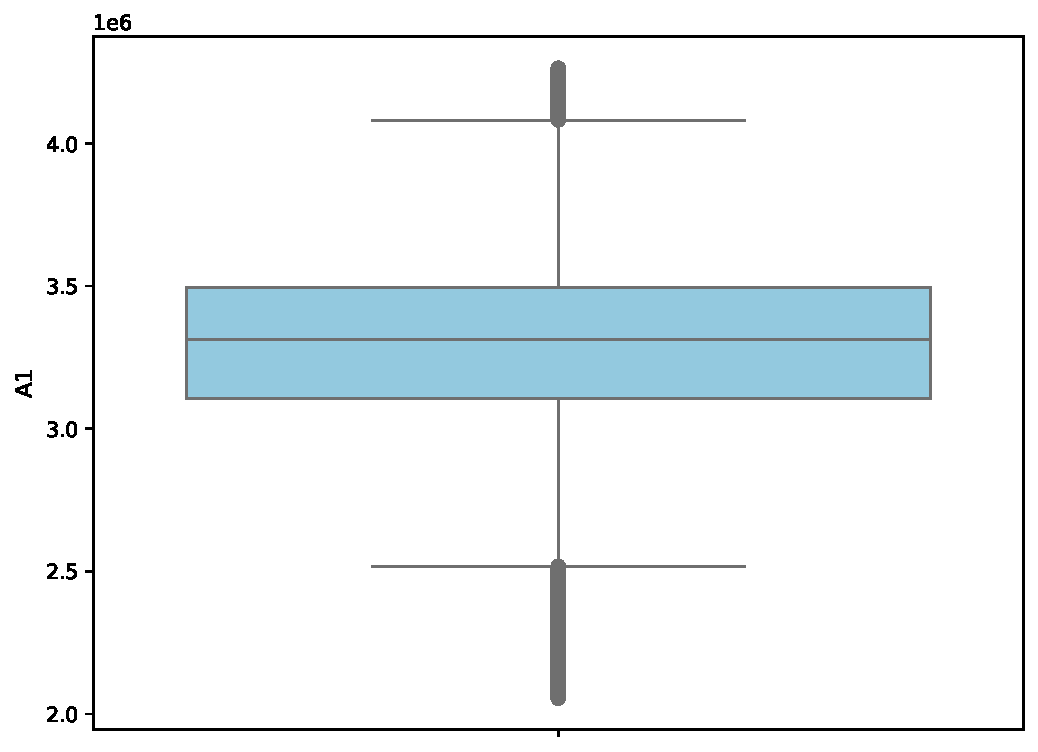
\includegraphics[width=0.6\textwidth]{images/A1_boxplot.pdf}
    \caption{Boxplot of A1.}
    \label{fig:a1_boxplot}
\end{figure}

The boxplot in figure~\ref{fig:a1_boxplot} provides a visual confirmation of the outliers in feature A1. The central box represents the interquartile range (IQR), containing the middle 50\% of the data. The points extending far below and above the whiskers of the box are individual data points identified as outliers. This visualization clearly shows that a significant number of outliers exist at both the lower and upper ends of the distribution.

\begin{figure}[H]
    \centering
    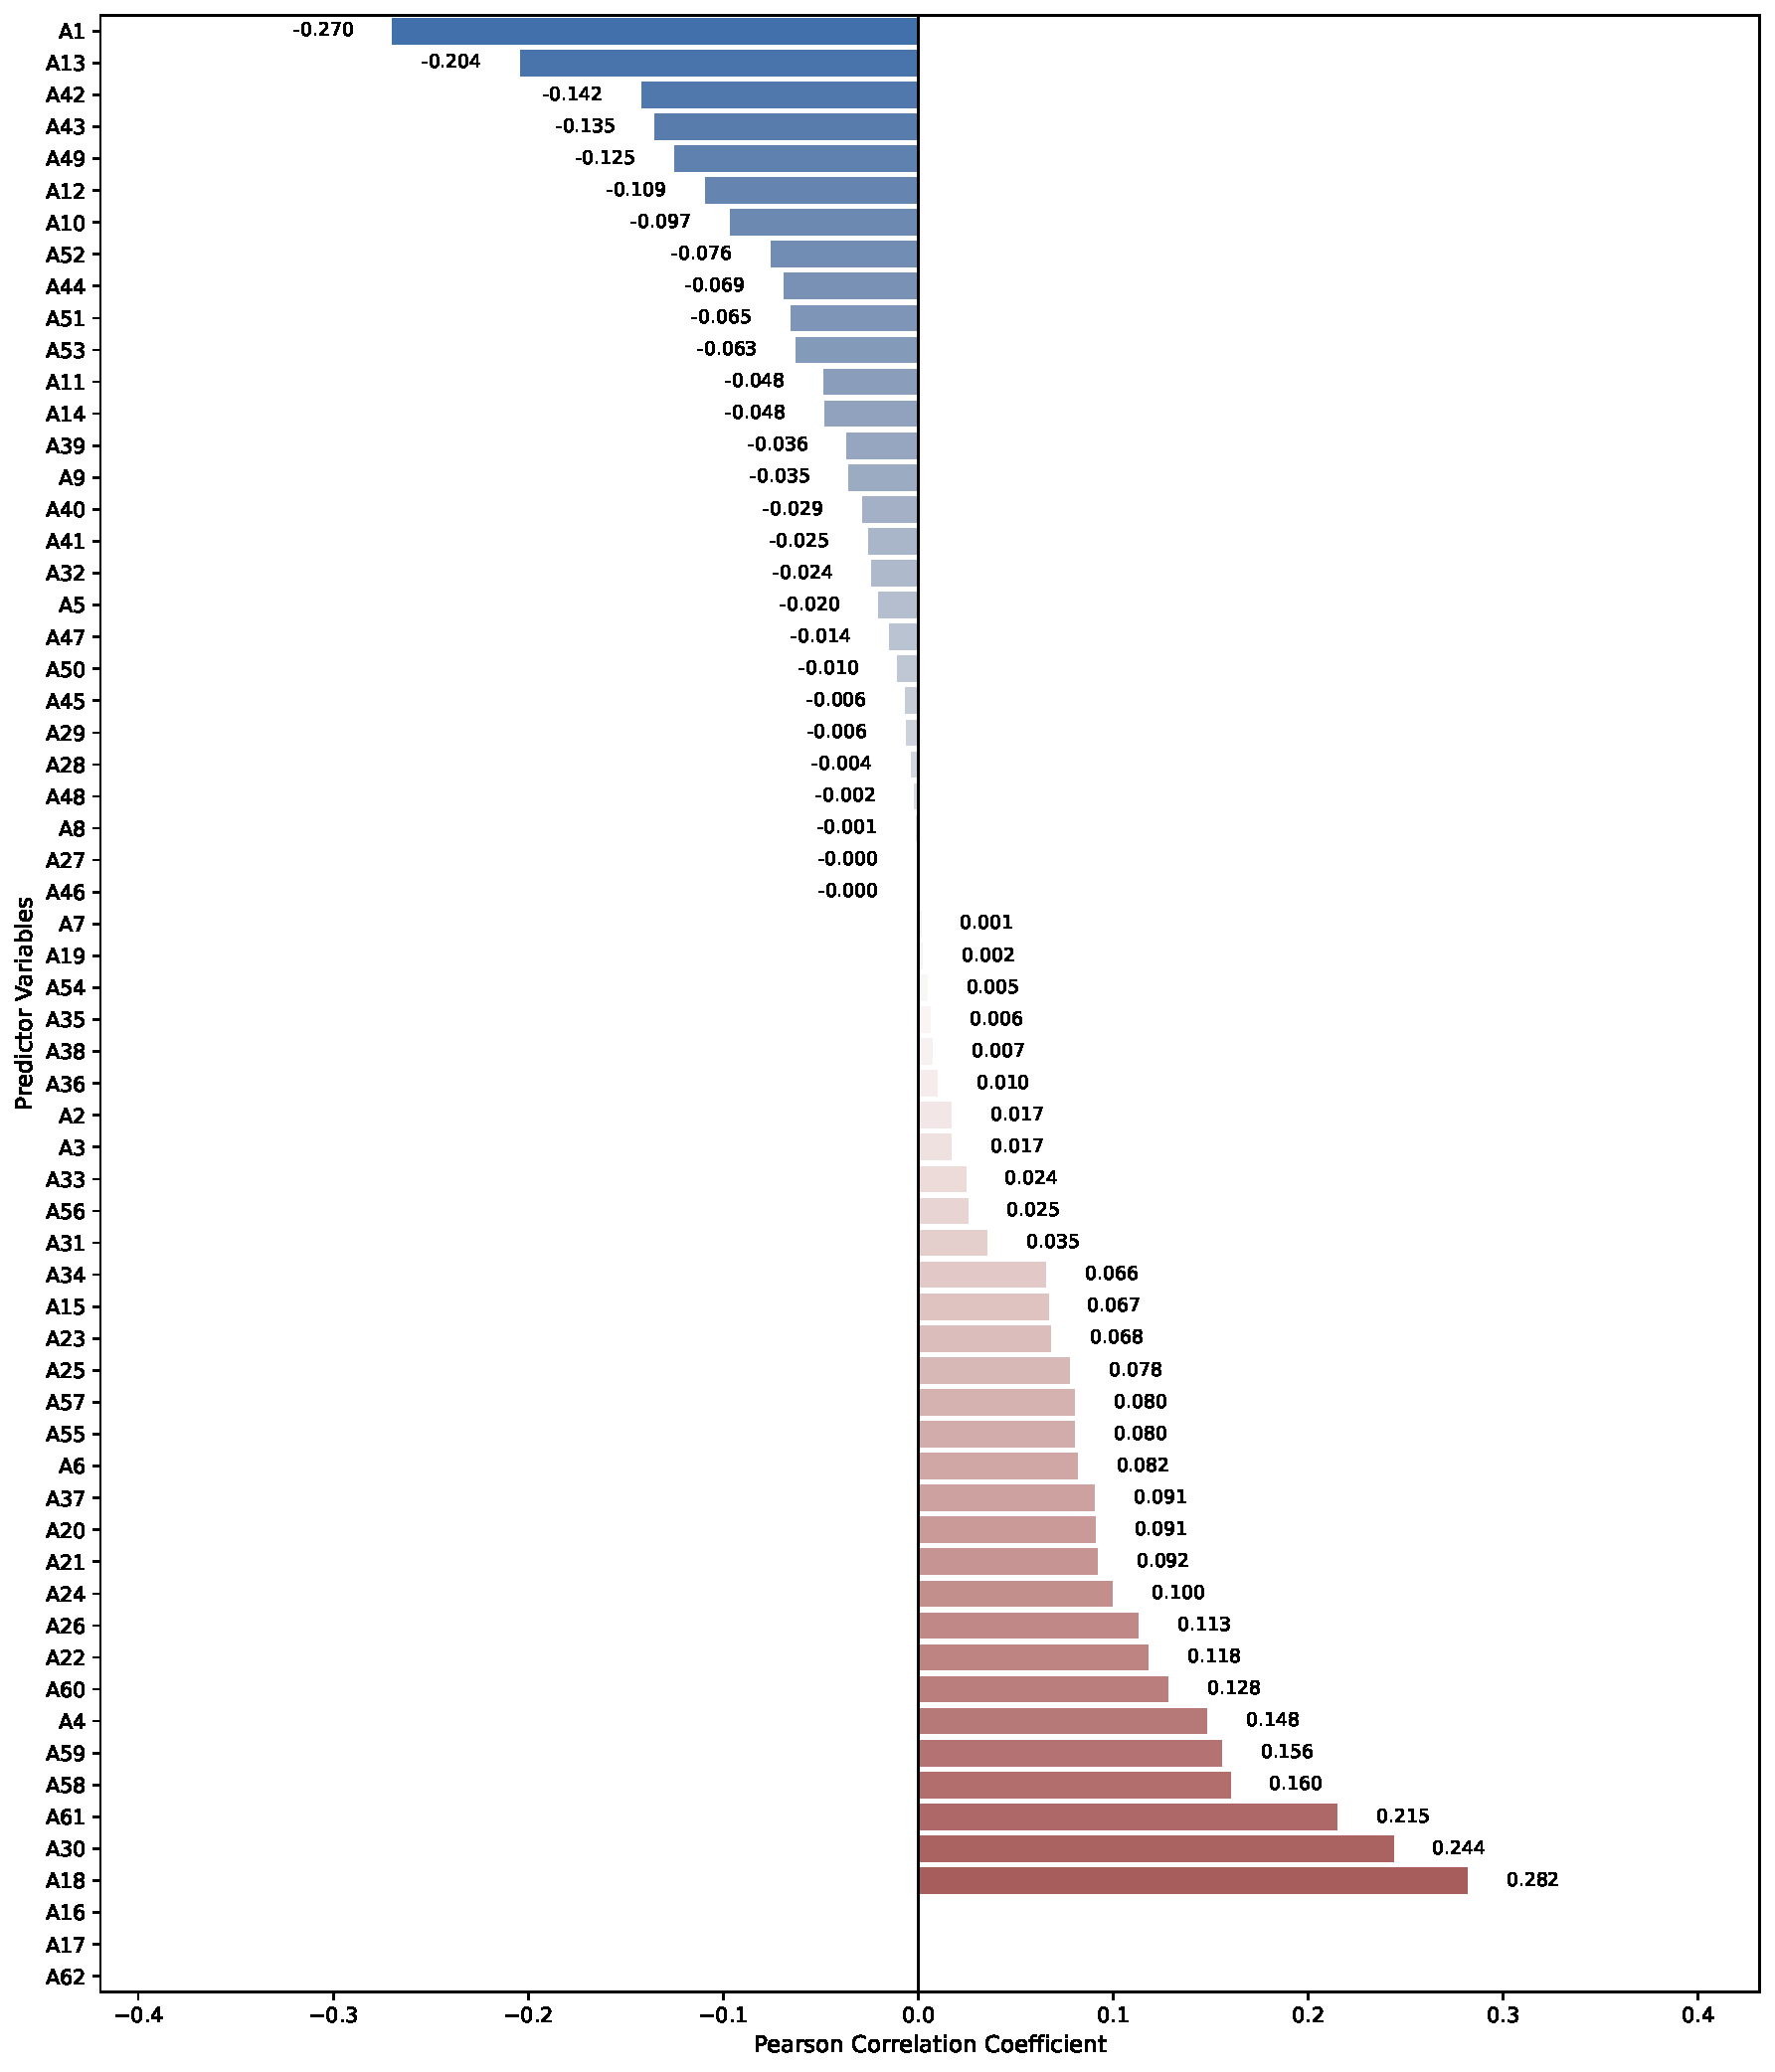
\includegraphics[width=0.6\textwidth]{images/correlation_with_T.pdf}
    \caption{Correlation of Each Predictor with Response Variable.}
    \label{fig:correlation_with_T}
\end{figure}

Figure~\ref{fig:correlation_with_T} illustrates the Pearson correlation coefficient, which measures the linear relationship between each predictor and the response. The analysis shows that most features have a weak to moderate correlation with the response, with all values falling between -0.27 and 0.29. This indicates that no single feature is a dominant predictor, suggesting that an effective model will need to leverage a combination of multiple features.

\begin{figure}[H]
    \centering
    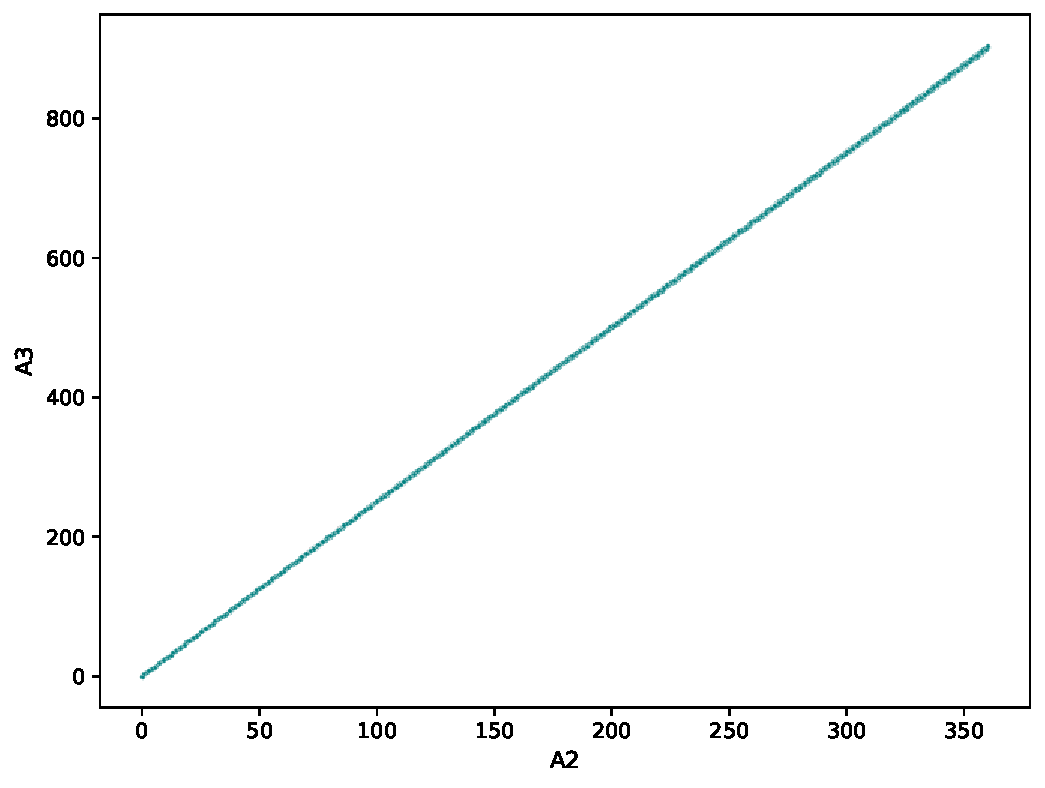
\includegraphics[width=0.6\textwidth]{images/A2_vs_A3_scatterplot.pdf}
    \caption{Scatterplot of A2 vs A3.}
    \label{fig:A2_vs_A3_scatterplot}
\end{figure}

Figure~\ref{fig:A2_vs_A3_scatterplot} shows that there is an extremely strong, positive, and linear relationship between A2 and A3. The line appears to start at the origin which indicates that A3 is just be a scaled version of A2. This means that the two variables are redundant and including both in the dataset does not provide any new information.

\begin{figure}[H]
    \centering
    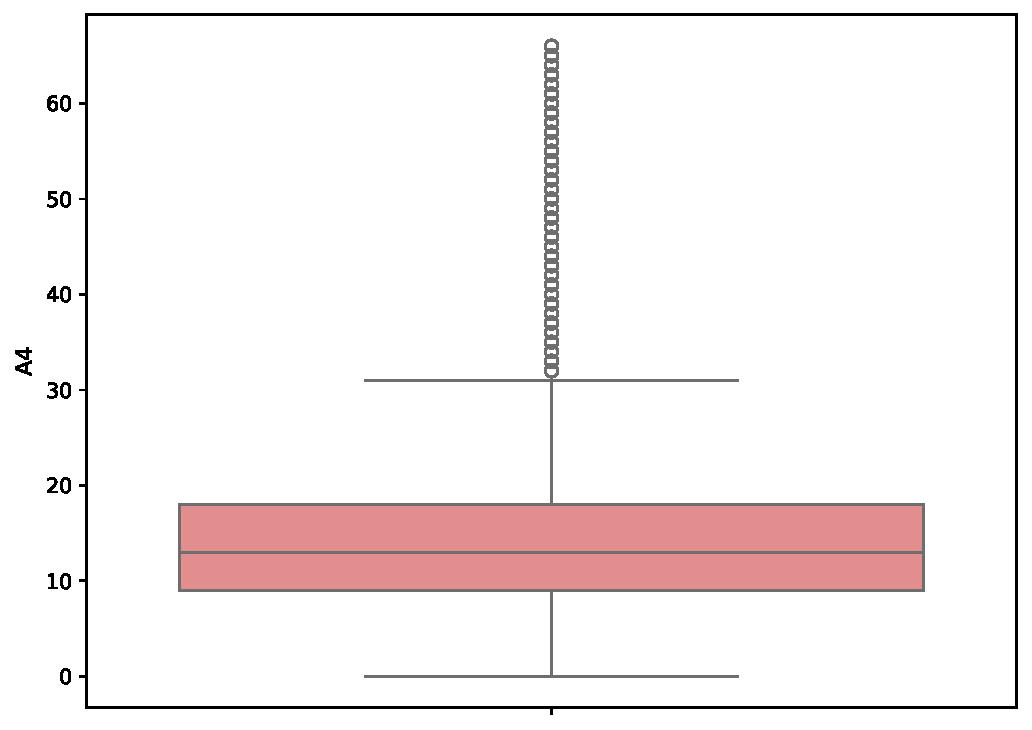
\includegraphics[width=0.6\textwidth]{images/A4_boxplot.pdf}
    \caption{Boxplot of A4.}
    \label{fig:a4_boxplot}
\end{figure}

The boxplot in figure~\ref{fig:a4_boxplot} shows that A4 has outliers in the upper range of its distribution.

\begin{figure}[H]
    \centering
    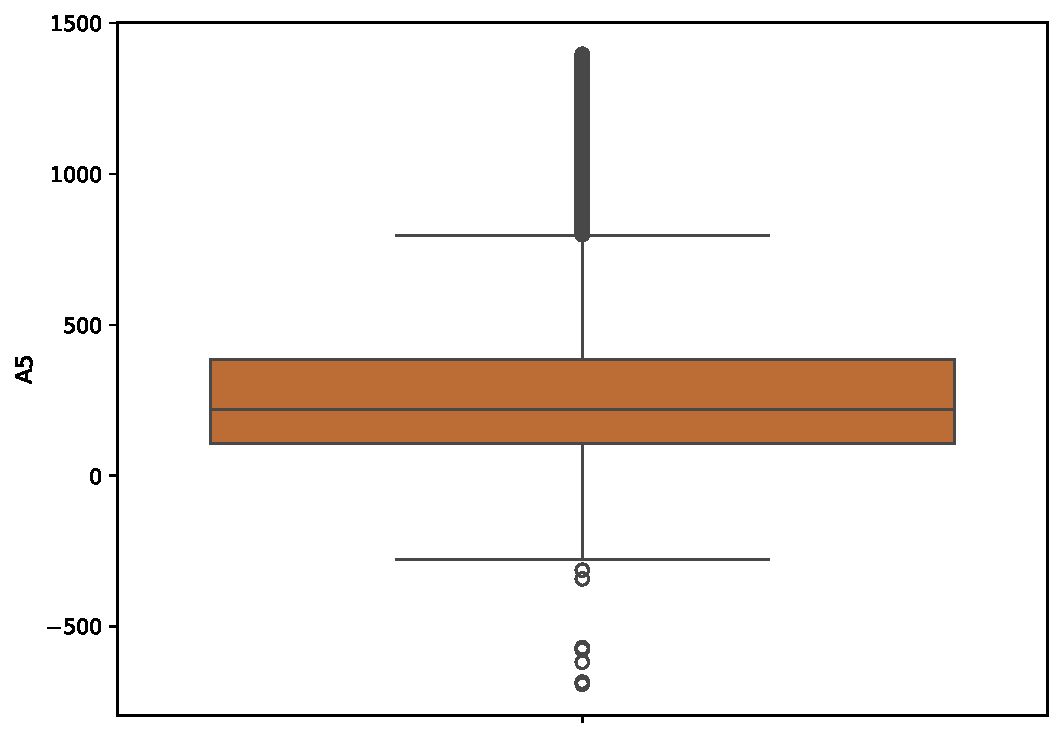
\includegraphics[width=0.6\textwidth]{images/A5_boxplot.pdf}
    \caption{Boxplot of A5.}
    \label{fig:a5_boxplot}
\end{figure}

The boxplot in figure~\ref{fig:a5_boxplot} shows that A5 has outliers in the lower and upper range of its distribution. A5 has quite a lot of outliers on the upper end compared to only a few on the lower end.

\begin{figure}[H]
    \centering
    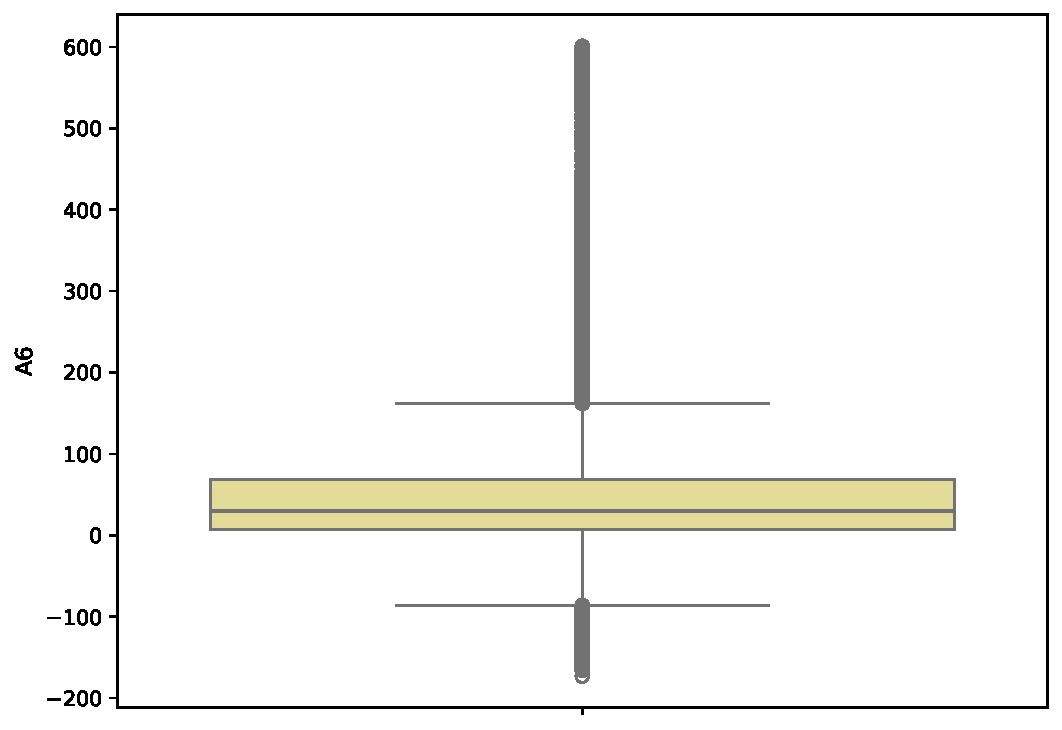
\includegraphics[width=0.6\textwidth]{images/A6_boxplot.pdf}
    \caption{Boxplot of A6.}
    \label{fig:a6_boxplot}
\end{figure}

The plot boxplot in figure~\ref{fig:a6_boxplot} shows that A6 has quite a few outliers, in both the lower and upper ends of its distribution.

\begin{figure}[H]
    \centering
    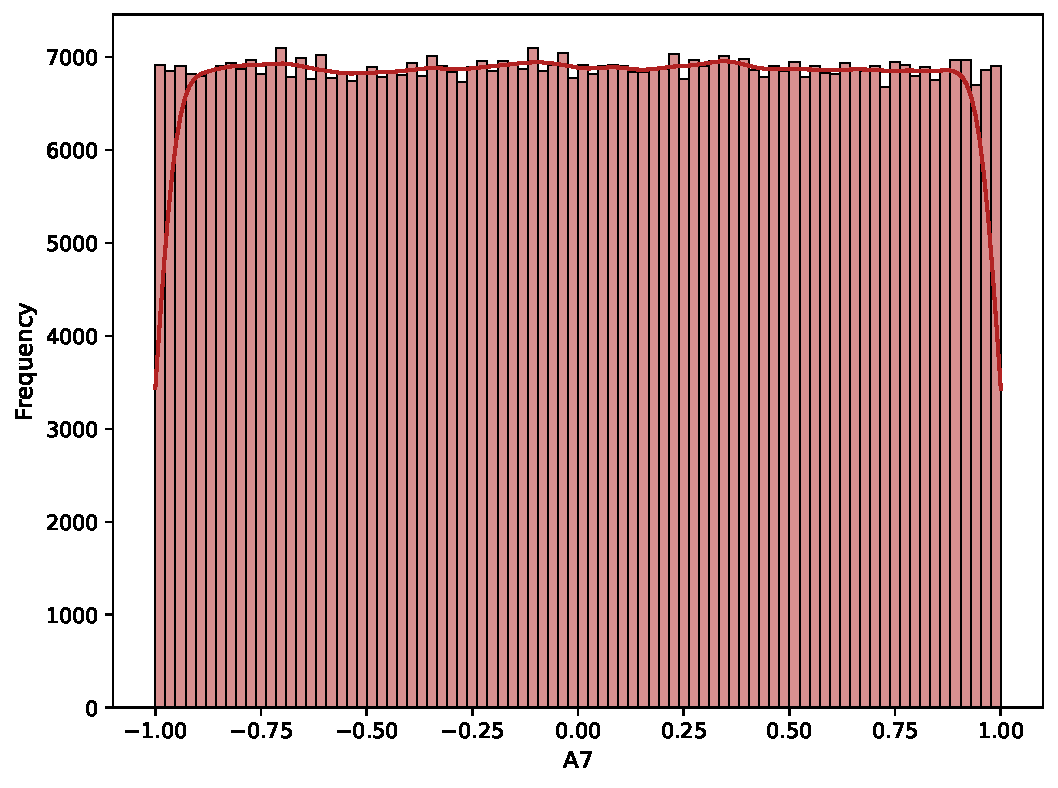
\includegraphics[width=0.6\textwidth]{images/A7_histplot.pdf}
    \caption{Histogram of A7.}
    \label{fig:a7_histplot}
\end{figure}

The histogram in figure~\ref{fig:a7_histplot} shows the distribution of A7. It indicates that A7 has an approximately uniform distribution over the range [-1, 1]. Since it also has high cardinality and a correlation of 0 with the response, feature A7 likely does not provide any useful information and including it in this dataset will likely harm any model trained on this dataset.

\begin{figure}[H]
    \centering
    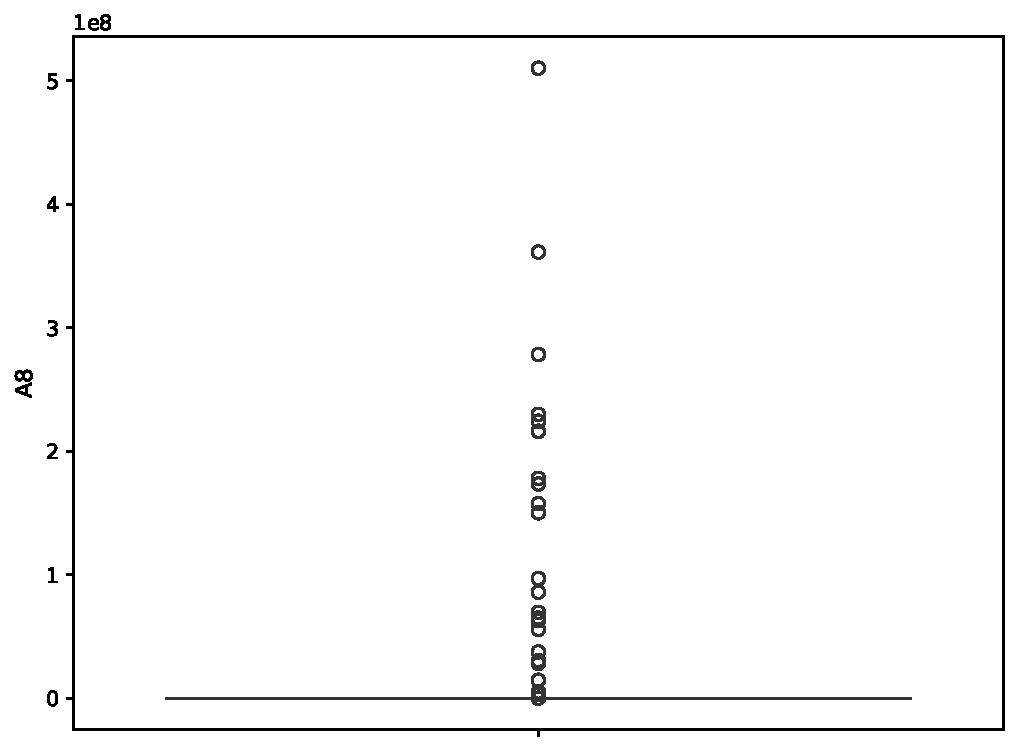
\includegraphics[width=0.6\textwidth]{images/A8_boxplot.pdf}
    \caption{Boxplot of A8.}
    \label{fig:a8_boxplot}
\end{figure}

\begin{figure}[H]
    \centering
    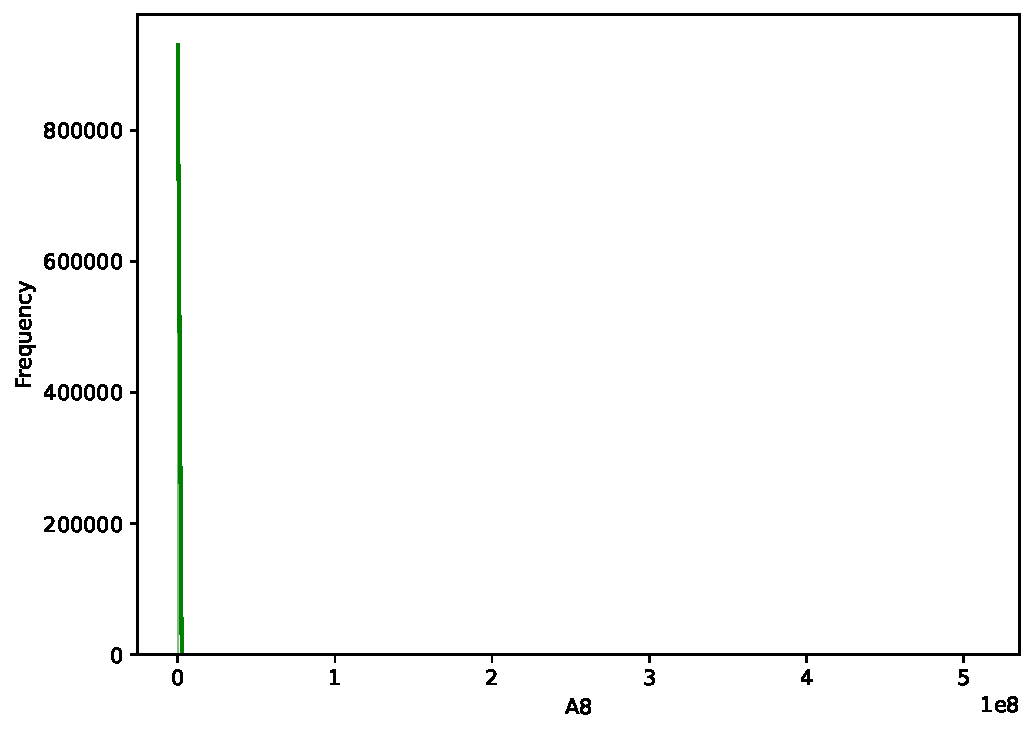
\includegraphics[width=0.6\textwidth]{images/A8_histplot.pdf}
    \caption{Histogram of A8.}
    \label{fig:a8_histplot}
\end{figure}

The boxplot in figure~\ref{fig:a8_boxplot} shows the extreme outliers in the higher end of the distribution of A8. The boxplot and the histogram in figure~\ref{fig:a8_histplot} show that these outliers cause A8 to have an extremely right skewed distribution. Although there are only a few outliers, they drastically affect the distribution of A8.

\begin{figure}[H]
    \centering
    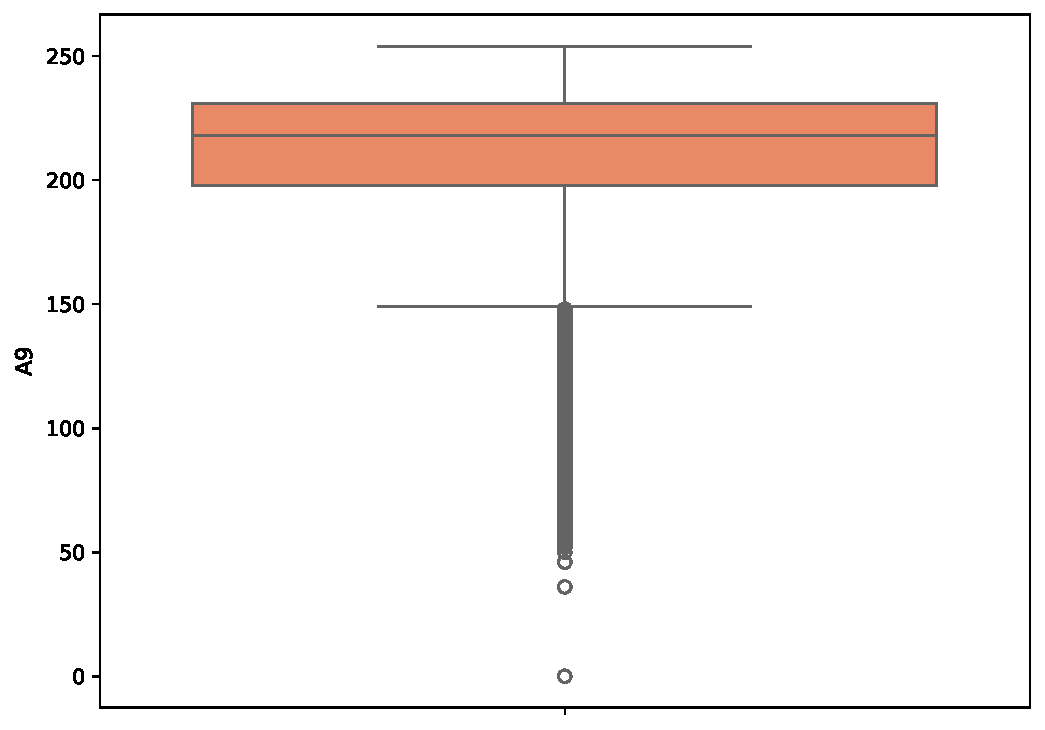
\includegraphics[width=0.6\textwidth]{images/A9_boxplot.pdf}
    \caption{Boxplot of A9.}
    \label{fig:a9_boxplot}
\end{figure}

The boxplot in figure~\ref{fig:a9_boxplot} shows that A9 has a bunch of outliers in the lower end of its distribution.

\begin{figure}[H]
    \centering
    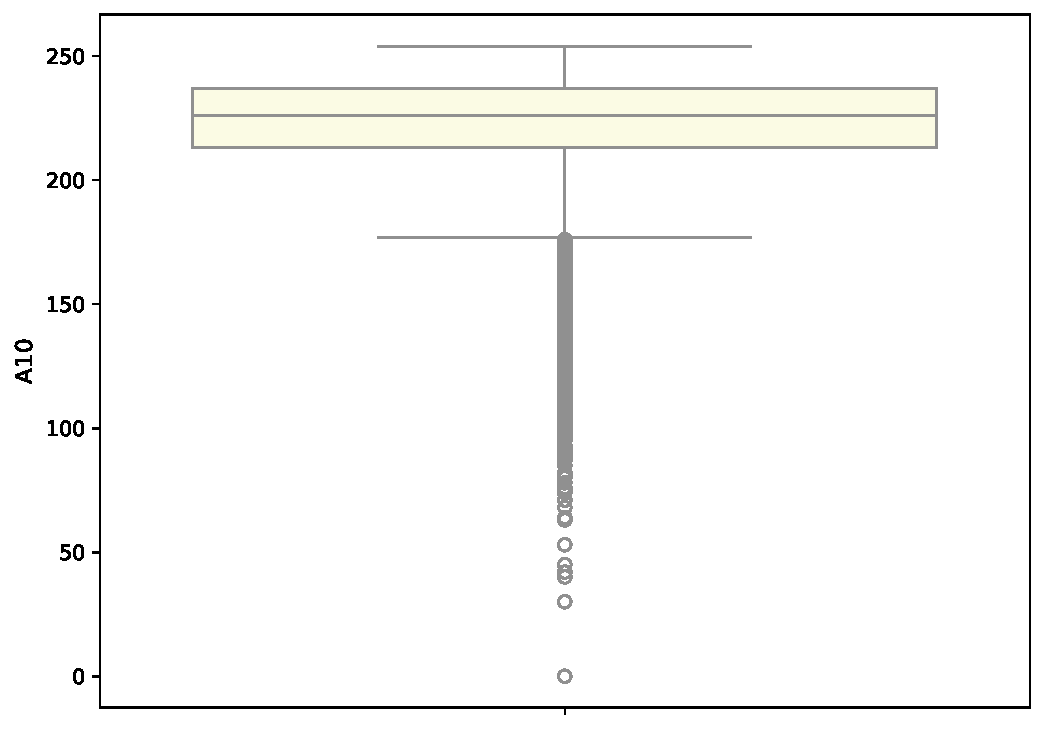
\includegraphics[width=0.6\textwidth]{images/A10_boxplot.pdf}
    \caption{Boxplot of A10.}
    \label{fig:a10_boxplot}
\end{figure}

The boxplot in figure~\ref{fig:a10_boxplot} was drawn after preprocessing A10, and treating all instances that are not numeric, meaning all instances of \textit{a}, as missing values. This plot shows that A10 has outliers in the lower end of its distribution.

\begin{figure}[H]
    \centering
    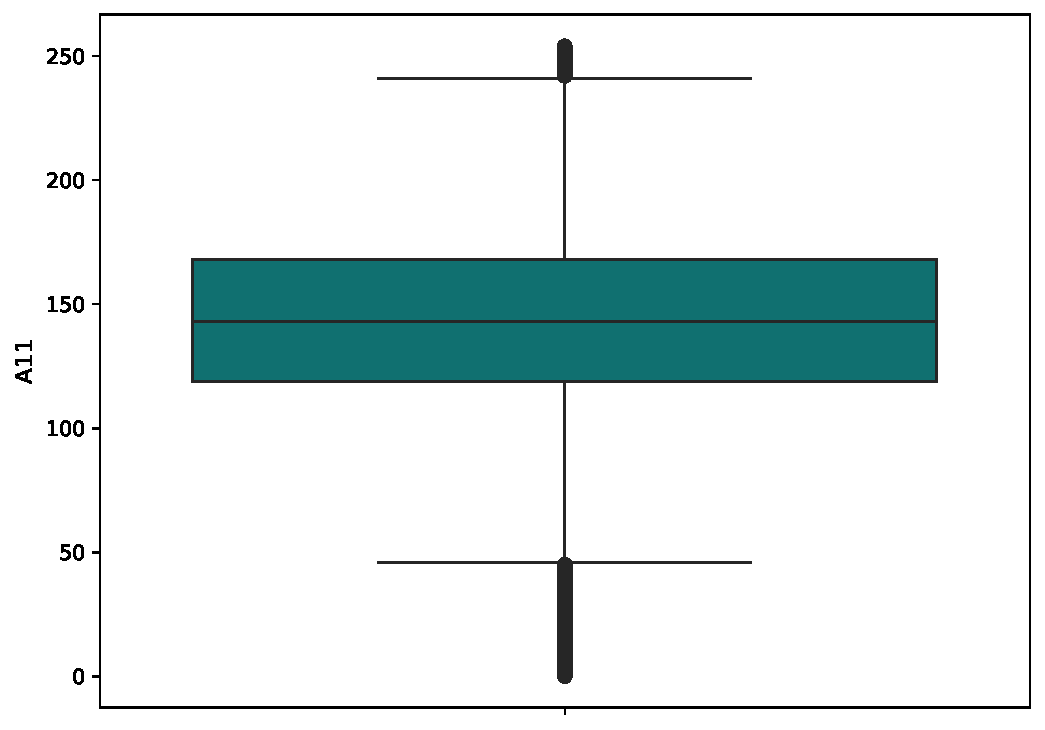
\includegraphics[width=0.6\textwidth]{images/A11_boxplot.pdf}
    \caption{Boxplot of A11.}
    \label{fig:a11_boxplot}
\end{figure}

The boxplot in figure~\ref{fig:a11_boxplot} shows that A11 has numerous outliers in both the lower and upper ranges of its distribution.

\begin{figure}[H]
    \centering
    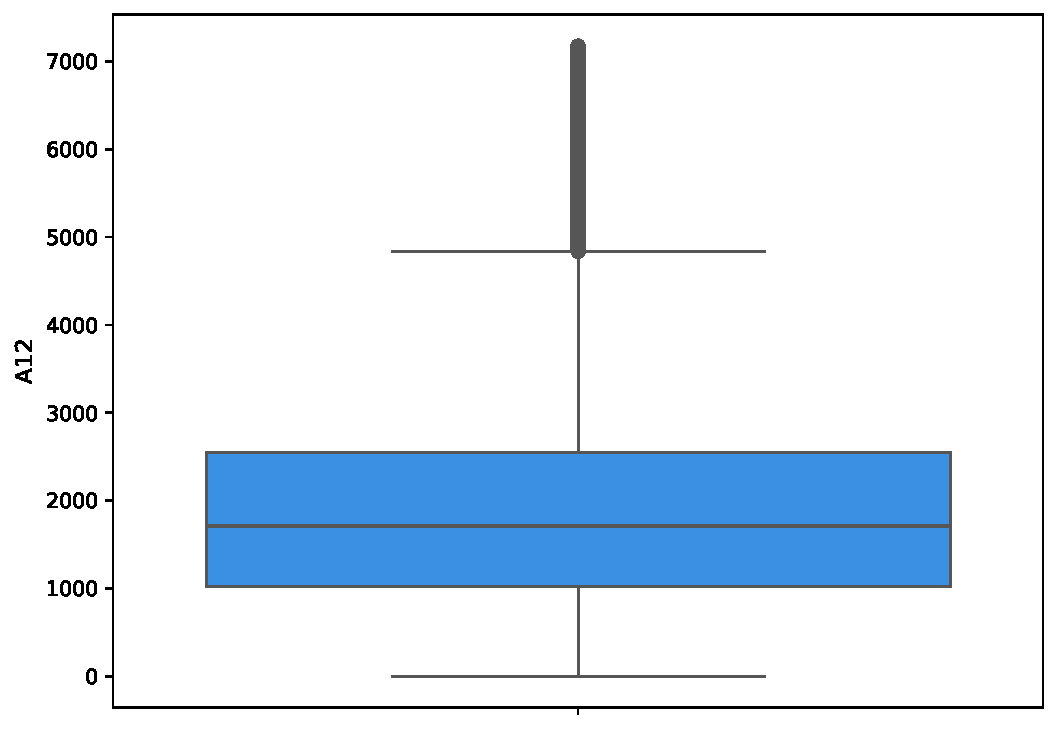
\includegraphics[width=0.6\textwidth]{images/A12_boxplot.pdf}
    \caption{Boxplot of A12.}
    \label{fig:a12_boxplot}
\end{figure}

The boxplot in figure~\ref{fig:a12_boxplot} indicates that A12 has numerous outliers in the upper end of its distribution.

\begin{figure}[H]
    \centering
    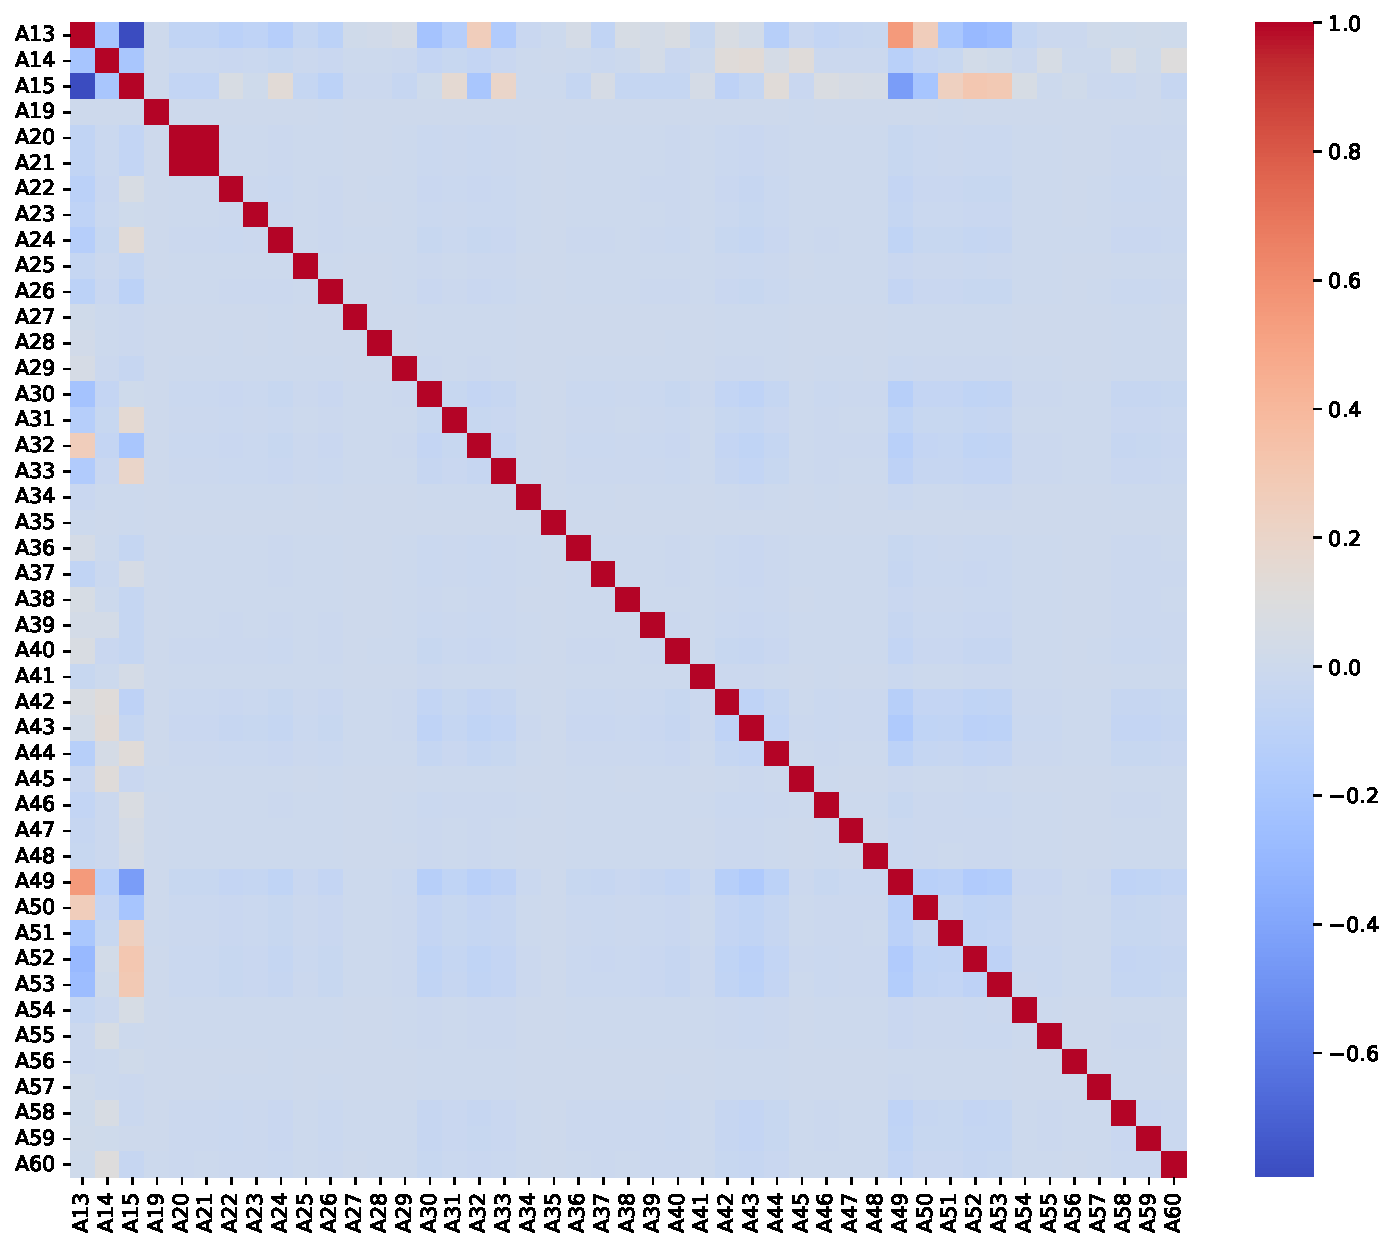
\includegraphics[width=0.7\textwidth]{images/binary_heatmap.pdf}
    \caption{Heat Map of Binary Features.}
    \label{fig:binary_heatmap}
\end{figure}

The heatmap in figure~\ref{fig:binary_heatmap} strongly suggests the presence of two groups of one-hot encoded variables. Binary one-hot encoded features created from the same original categorical variable are inherently negatively correlated. This means that distinct blocks of blue (negatively correlated) squares in the heatmap in figure~\ref{fig:binary_heatmap} correspond to encodings of a distinct original categorical variable. A13, A14, \& A15 are the first group, since they are all negatively correlated with one another. A19-A60 is another group of one-hot encoded variables as they are also negatively correlated with one another. There is correlation present between the variables in the first and second group, which also strongly suggests that these are groups of two distinct one-hot encoded categorical features.

\end{document}